\documentclass[tikz,border=10pt]{standalone}
\usepackage{tikz}
\usetikzlibrary{shapes, arrows.meta, positioning, fit, calc, backgrounds, shadows}
\usepackage{amsmath, amssymb}
\usepackage{newtxtext,newtxmath} 

% ==========================================
%  1. 语义化配色定义
% ==========================================
\definecolor{cThreadFill}{RGB}{225, 245, 254}
\definecolor{cThreadDraw}{RGB}{2, 119, 189}
\definecolor{cSyncFill}{RGB}{224, 242, 241}
\definecolor{cSyncDraw}{RGB}{0, 105, 92}
\definecolor{cDataFill}{RGB}{255, 243, 224}
\definecolor{cDataDraw}{RGB}{239, 108, 0}
\definecolor{cHwFill}{RGB}{245, 245, 245}
\definecolor{cHwDraw}{RGB}{66, 66, 66}
\definecolor{bgLayerScope}{RGB}{240, 244, 248} 
\definecolor{bgLayerMem}{RGB}{255, 255, 255}   
\definecolor{lineColor}{RGB}{60, 60, 60}       

% ==========================================
%  2. 样式设置 (Styles)
%  注意:tikzset 内部严禁出现完全空白的行,必须用 % 注释占位
% ==========================================
\tikzset{
    node distance=1.0cm and 1.0cm,
    font=\footnotesize\sffamily,
    % --- 基础块样式 ---
    baseBlock/.style={
        rectangle, thick, rounded corners=3pt,
        minimum width=2.5cm, minimum height=1.2cm, 
        align=center,
        drop shadow={opacity=0.1, shadow xshift=1pt, shadow yshift=-1pt}
    },
    % --- 语义样式 ---
    styleThread/.style={baseBlock, draw=cThreadDraw, fill=cThreadFill, font=\footnotesize\bfseries},
    styleSync/.style={baseBlock, draw=cSyncDraw, fill=cSyncFill, font=\ttfamily\footnotesize},
    styleData/.style={baseBlock, draw=cDataDraw, fill=cDataFill, line width=1.0pt},
    styleHw/.style={baseBlock, draw=cHwDraw, fill=cHwFill, font=\scriptsize},
    % --- 虚线框 ---
    styleScope/.style={
        rectangle, draw=black!30, dashed, fill=bgLayerScope,
        inner sep=10pt, rounded corners=5pt
    },
    % --- 连线样式 ---
    conn/.style={
        draw=lineColor, line width=0.9pt,
        -{Latex[length=2.5mm, width=1.5mm]}
    },
    connDashed/.style={
        conn, dashed
    },
    % --- 小图标定义 ---
    threadIcon/.pic = {
        \draw[lineColor, thick, smooth] (-0.3,0) sin (-0.15,0.15) cos (0,0) sin (0.15,-0.15) cos (0.3,0);
    },
    lockIcon/.pic = {
        \draw[lineColor, fill=white, thick] (-0.15, -0.12) rectangle (0.15, 0.15);
        \draw[lineColor, thick] (-0.1, 0.15) arc (180:0:0.1);
    }
}

\begin{document}
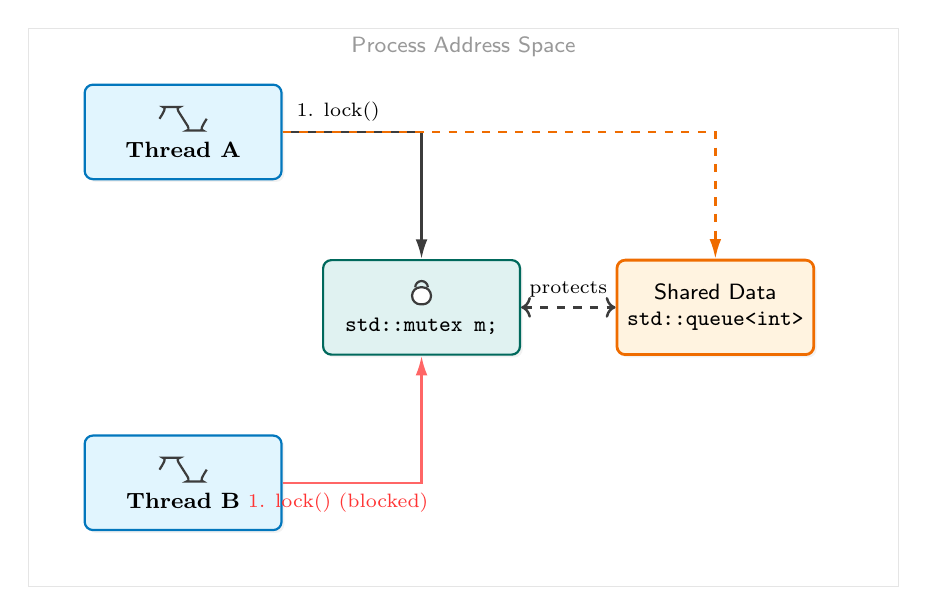
\begin{tikzpicture}

    % =========================================================
    % 3. 示例布局
    % =========================================================

    % Mutex
    \node [styleSync] (mutex) {
        \tikz\pic[scale=0.8, yshift=3pt]{lockIcon}; \\
        std::mutex m;
    };

    % Data
    \node [styleData, right=1.2cm of mutex] (data) {
        Shared Data\\
        \texttt{std::queue<int>}
    };

    % Thread A
    \node [styleThread, above left=1.0cm and 0.5cm of mutex] (threadA) {
        \tikz\pic[scale=1.0, xshift=-15pt]{threadIcon}; \\ Thread A
    };
    
    % Thread B
    \node [styleThread, below left=1.0cm and 0.5cm of mutex] (threadB) {
        \tikz\pic[scale=1.0, xshift=-15pt]{threadIcon}; \\ Thread B
    };

    % =========================================================
    % 4. 连线
    % =========================================================

    % Thread A 逻辑
    \draw [conn] (threadA.east) -| node[pos=0.2, above, font=\scriptsize] {1. lock()} (mutex.north);
    \draw [conn, dashed, draw=cDataDraw] (threadA.east) -| (data.north);
    
    % Thread B 逻辑
    \draw [conn, draw=red!60] (threadB.east) -| node[pos=0.2, below, font=\scriptsize, text=red!80] {1. lock() (blocked)} (mutex.south);

    % Mutex 保护关系
    \draw [connDashed, <->] (mutex) -- node[above, font=\scriptsize] {protects} (data);

    % =========================================================
    % 5. 背景层
    % =========================================================
    
    \begin{scope}[on background layer]
        % 临界区
        \node [styleScope, fit=(mutex) (data), 
            label={[anchor=north west, text=black!60, font=\scriptsize]north west:Critical Section}] (criticalSection) {};
            
        % 进程空间
        \node [draw=black!10, fill=white, fit=(threadA) (threadB) (criticalSection), inner sep=20pt, z=-1,
             label={[anchor=north, text=black!40]north:Process Address Space}] {};
    \end{scope}

\end{tikzpicture}
\end{document}